%!TEX root = lec06_transactions.tex


%
% -----------------------------------------------
%
\begin{frame}{Concurrent access to the database}
\begin{center}
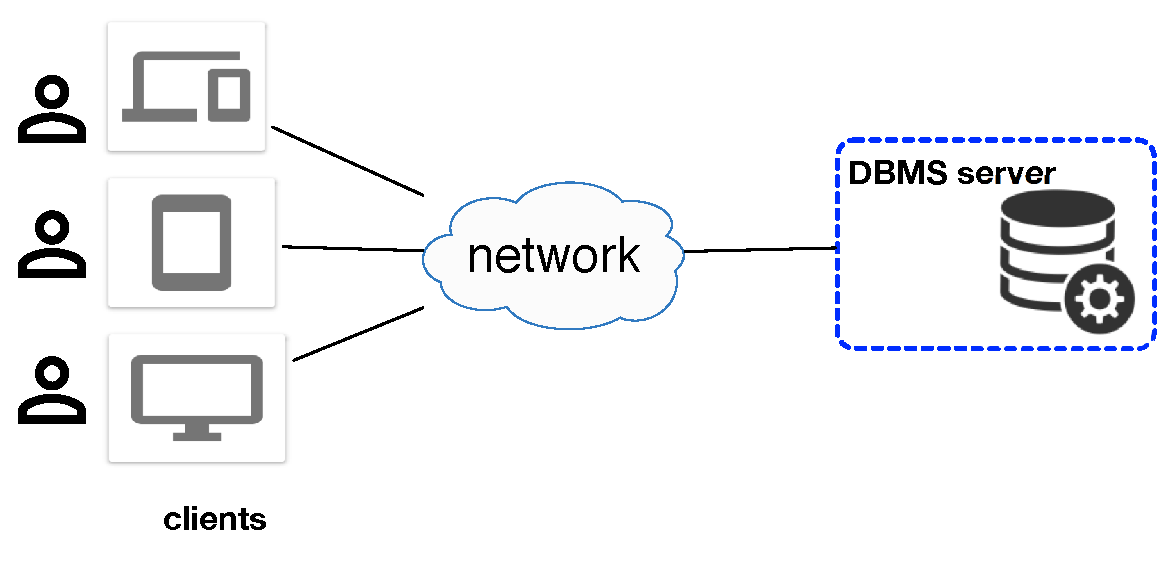
\includegraphics[width=0.75\textwidth]{../lec03_hardware/figures/client_server_cloud}
\end{center}

Most databases are used concurrently by many users (e.g., think of Bear Tracks), posing a mix of queries and updates at the same time.

The DBMS must decide the order in which the transactions (queries or updates) are executed, ensuring the integrity of the data at all times.

\end{frame}

\newsavebox\serialExecutionTimeline
\savebox{\serialExecutionTimeline}{%
\footnotesize
\begin{tabular}{ll|rr}
$T_1$ & $T_2$ & \texttt{A} & \texttt{B} \\
\hline
& & 75 & 40 \\
\READ{A}{v}; \ASSIGN{v}{v-20} & & & \\
\WRITE{A}{v} & & \alert{55} & \\
\READ{B}{v}; \ASSIGN{v}{v+20} & & &  \\
\WRITE{B}{v} & & & \alert{60} \\
\COMMIT & & 55 & 60 \\
& \READ{B}{t}; \ASSIGN{t}{t*1.1} & & \\
& \WRITE{B}{t} & & \alert{66} \\
& \COMMIT  & 55 & 66 \\
\end{tabular}
}

\newsavebox\serialExecutionTimelineII
\savebox{\serialExecutionTimelineII}{%
\footnotesize
\begin{tabular}{ll|rr}
$T_1$ & $T_2$ & \texttt{A} & \texttt{B} \\
\hline
& & 75 & 40 \\
& \READ{B}{t}; \ASSIGN{t}{t*1.1} & & \\
& \WRITE{B}{t} & & \alert{44} \\
& \COMMIT  & 75 & 44 \\
\READ{A}{v}; \ASSIGN{v}{v-20} & & & \\
\WRITE{A}{v} & & \alert{55} & \\
\READ{B}{v}; \ASSIGN{v}{v+20} & & &  \\
\WRITE{B}{v} & & & \alert{64}\\
\COMMIT & & 55 & 64 \\
\end{tabular}
}


%
% -----------------------------------------------
%
\begin{frame}{Running example}

Assume we have two transactions now:
\begin{itemize}[-,noitemsep]
 \item $T_1$ transfers from checking into investment as before; and
 \item $T_2$ accrues 10\% interest in the investment. 
\end{itemize}

\vskip1em

The correct execution of the transactions now goes beyond ensuring atomicity with the help of the log. 

Because the two transactions modify the same database element (the balance in the investment account), we say there is a \alert{race condition} between them.

If both transaction attempt to modify it concurrently, the DBMS needs to decide who gets to modify that element first, in a way that the account holder does not lose money.

\end{frame}


%
% -----------------------------------------------
%
\begin{frame}

\begin{block}{Serial Schedule}
A schedule of two or more transactions is \textbf{serial} if every transaction executes to completion before the next transaction starts.
\end{block}

\vskip2em

\begin{center}
\scalebox{0.9}{\usebox{\serialExecutionTimeline}}
\end{center}

\vskip1em

\underline{Ideal form of \alert{isolation}}: if no two transactions overlap, they cannot interfere with one another.
\end{frame}


\begin{frame}

Serial execution of transactions \alert{is not the same} as \emph{deterministic} execution of transactions:
\begin{itemize}[-,noitemsep]
\item If there are two or more transactions ready for execution, the order in which they are picked determines the outcome.
\end{itemize}

\vskip2em

\begin{center}
\scalebox{0.9}{\usebox{\serialExecutionTimelineII}}
\end{center}

\end{frame}

%
% -----------------------------------------------
%
\begin{frame}{Why add concurrency?}

Allowing multiple transactions to run concurrently brings opportunities for parallelism, which leads to faster response times for the users:

\begin{itemize}[-,topsep=-0.5em]
\item E.g., while one transaction waits for user input (e.g., credit card information), another transaction can use the CPU.
\end{itemize}


\vskip1.5em

\textbf{Conflicting Goals:}
\begin{enumerate}[(1),topsep=-0.5em]
  \item Users want as much parallelism and concurrency as possible.
  \item As long as it does not interfere with their work.
\end{enumerate}
\end{frame}


\newsavebox\lostUpdateTimeline
\savebox{\lostUpdateTimeline}{%
\footnotesize
\begin{tabular}{ll|rr}
$T_1$ & $T_2$ & \texttt{A} & \texttt{B} \\
\hline
& & 75 & 40   \\
\READ{A}{v}; \ASSIGN{v}{v-20} & & &   \\
\WRITE{A}{v} & & 55 \\
\READ{B}{v}; \ASSIGN{v}{v+20} & & &\\
& \READ{B}{t}; \ASSIGN{t}{t*1.1} & & \\
& \WRITE{B}{t} & &  44\\
& \COMMIT \\
\WRITE{B}{V} & & & 60 \\
\COMMIT & & 55 & 60\\
\end{tabular}
}

%
% -----------------------------------------------
%
\begin{frame}{Problems with uncontrolled concurrency}

\textbf{\#1}: the lost update problem.

Happens when a transaction overwrites the changes made by another.

\vskip1em

\begin{center}
\begin{tikzpicture}[semithick,every node/.append style={font=\footnotesize}]
\node[anchor=south west,inner sep=0pt,outer sep=0pt] at (0,0) {\scalebox{0.9}{\usebox{\lostUpdateTimeline}}};
\only<2 | handout:1>{
\begin{scope}[on background layer]
  \draw[orange!50] [fill=orange!10] (3.5,0.8) rectangle (8.5,2);
  \node (l) at (6,3) [red] {lost transaction};
  \draw[->,very thick,orange] (l) -- (6,2);
\end{scope}}
\end{tikzpicture}
\end{center}
\end{frame}

\newsavebox\dirtyReadTimeline
\savebox{\dirtyReadTimeline}{%
\footnotesize
\begin{tabular}{ll|rr}
$T_1$ & $T_2$ & \texttt{A} & \texttt{B} \\
\hline
& & 75 & 40 \\
\READ{A}{v}; \ASSIGN{v}{v-20} & & & \\
\WRITE{A}{v} & & 55 \\
& \READ{B}{t}; \ASSIGN{t}{t*1.1} & & \\
& \WRITE{B}{t} & &  44 \\
\READ{B}{v}; \ASSIGN{v}{v+20} & & \\
& \ABORT & & \\
\WRITE{B}{v} & & & 64 \\
\COMMIT & & & \\
& & 55 & 64 \\
\end{tabular}
}

%
% -----------------------------------------------
%
\begin{frame}

\textbf{\# 2}: the uncommitted dependency problem.

Happens when a transaction is allowed to update an element using an uncommitted value of another element written by a transaction that later one aborts.

\vskip1em

\begin{center}
\begin{tikzpicture}[semithick]
\node[anchor=south west,inner sep=0pt,outer sep=0pt] at (0,0) {\scalebox{0.9}{\usebox{\dirtyReadTimeline}}};
\only<2 | handout:1>{
\begin{scope}[on background layer]
  \draw[orange!50] [fill=orange!10] (0.125,1.6) rectangle (1.9,2.1);
  \draw[red!50] [fill=red!10] (3.5,1.9) rectangle (5.25,2.4);
  \draw[<-,thick,red] plot [smooth] coordinates { (0.9, 2.1) (2.1,2.3) (3.5,2.1)};
  \node at (2.1,2.5) [red] {\tiny dirty read};
\end{scope}}
\end{tikzpicture}
\end{center}
\end{frame}


\newsavebox\inconsistentAnalysisTimeline
\savebox{\inconsistentAnalysisTimeline}{%
\footnotesize
\begin{tabular}{ll|rr||c}
$T_1$ & $T_3$ & \texttt{A} & \texttt{B} & \lstinline[style=SQL]!SUM! \\
\hline
 & & 75 & 40 & \\
\READ{A}{v}; \ASSIGN{v}{v-20} & & & & \\
& \READ{A}{t}; \ASSIGN{sum}{t} & & & 75 \\
\WRITE{A}{v} & & 55 & \\
\READ{B}{v}; \ASSIGN{v}{v+20} & & & & \\
\WRITE{B}{v} & & & 60 & \\
\COMMIT & & 55 & 60 & \\
& \READ{B}{t}; \ASSIGN{sum}{sum+t} & & & \alert{135}\\
\end{tabular}
}

\begin{frame}[fragile]

\textbf{\# 3}: the inconsistent analysis problem.

Happens when a transaction and a query both read/write the same elements concurrently. 

\vskip1em

\begin{columns}[onlytextwidth]
\begin{column}{0.7\textwidth}
\textbf{Example:} transaction $T_3$, a query that returns the sum of all funds owned by Nuttah.

\end{column}

\begin{column}{0.25\textwidth}
\begin{lstlisting}[style=SQL]
SELECT SUM(balance)
FROM Account
WHERE holder=7564
\end{lstlisting}
\end{column}
\end{columns}

\begin{center}
\scalebox{0.9}{\usebox{\inconsistentAnalysisTimeline}}
\end{center}

\end{frame}


\section{Serializability}

%
% -----------------------------------------------
%
\begin{frame}

Since each transaction individually cannot cause the database to become inconsistent, a concurrent schedule of transactions $T_1,\ldots, T_k$ that does not cause inconsistencies must be \alert{equivalent} to a serial schedule of the same transactions\footnote{As we will see soon, this is true only if no transaction aborts.}.

Such a schedule is called \textbf{serializable}.

\vskip1em

\begin{block}{Testing \alert{serializability} of schedule $S$}
\begin{itemize}[-,noitemsep]
\item Draw a graph where every node is a transaction in $S$.
\item Add an edge from transaction $T_i$ to $T_j$ if:
\begin{itemize}[$\bullet$,noitemsep, topsep=-5pt]
\item $T_i$ and $T_j$ access the same element; 
\item at least one of them writes that element in common; 
\item $T_i$ performs its operation before $T_j$.
\end{itemize}
\item If the graph has a cycle, $S$ \textbf{\alert{is not serializable}}.
\end{itemize}
\end{block}

\end{frame}

%
% -----------------------------------------------
%
\begin{frame}{Examples}

Serializable schedule with funds transfer ($T_1$) before interest calculation ($T_2$).

\vskip2em

\begin{center}
\begin{tikzpicture}[->,>=stealth',shorten >=1pt,auto,node distance=2.5cm,semithick,every node/.append style={font=\footnotesize}]
\node[anchor=south west,inner sep=0pt,outer sep=0pt] at (0,1) {
\scalebox{0.9}{\clipbox{0pt 0pt 50pt 0pt}{\usebox{\serialExecutionTimeline}}}
};

\node[state] 	(1)  at (1,0)      {$T_1$};
\node[state]  (2) [right of=1]   {$T_2$};

\onslide<2- | handout:1>{
\begin{scope}[on background layer]
  \draw[red,fill=red!10] plot [smooth cycle] coordinates { (0.25, 2.6) (0.25,3.4) (1.8,3.4) (1.8,2.6)};
  \draw[blue,fill=blue!10] plot [smooth cycle] coordinates { (3.8, 1.4) (3.8,2.2) (5.35,2.2) (5.35,1.4)};
  \draw[->,thick,red] plot [smooth] coordinates { (2, 2.9) (4,2.8) (4.5,2.2)};
\end{scope}}

\onslide<3- | handout:1>{
  \path[->] (1) edge (2) ;
}
  
\end{tikzpicture}
\end{center}
\end{frame}

\newsavebox\serializableTIandTIII
\savebox{\serializableTIandTIII}{%
\footnotesize
\begin{tabular}{ll|rr||c}
$T_1$ & $T_3$ & \texttt{A} & \texttt{B} & \lstinline[style=SQL]!SUM! \\
\hline
 & & 75 & 40 & \\
& \READ{A}{t}; \ASSIGN{sum}{t} & & & 75 \\
\READ{A}{v}; \ASSIGN{v}{v-20} & & & & \\
\WRITE{A}{v} & & 55 & \\
& \READ{B}{t}; \ASSIGN{sum}{sum+t} & & & \alert{115}\\
\READ{B}{v}; \ASSIGN{v}{v+20} & & & & \\
\WRITE{B}{v} & & & 60 & \\
\COMMIT & & 55 & 60 & \\
\end{tabular}
}



\begin{frame}

Serializable schedule with funds transfer ($T_1$) concurrently with query ($T_3$).

\vskip2em

\begin{center}
\begin{tikzpicture}[->,>=stealth',shorten >=1pt,auto,node distance=2.5cm,semithick,every node/.append style={font=\footnotesize}]
\node[anchor=south west,inner sep=0pt,outer sep=0pt] at (0,1) {
\scalebox{0.9}{\clipbox{0pt 0pt 80pt 0pt}{\usebox{\serializableTIandTIII}}}
};

\node[state]  (1)  at (1,0)      {$T_1$};
\node[state]  (3) [right of=1]   {$T_3$};
\only<2- | handout:1>{
\begin{scope}[on background layer]
  \draw[red,fill=red!10] plot [smooth cycle] coordinates { (3.8, 3.4) (3.8,3.8) (5.35,3.8) (5.35,3.4)};
  \draw[blue,fill=blue!10] plot [smooth cycle] coordinates { (0.25, 2.6) (0.25,3) (1.8,3) (1.8,2.6)};
  \draw[->,thick,red] plot [smooth] coordinates {(4.5,3.4) (4,2.9) (2, 2.8)};
\end{scope}}

\only<3- | handout:1>{
\begin{scope}[on background layer]  
  \draw[red,fill=red!10] plot [smooth cycle] coordinates { (3.8, 2.2) (3.8,2.6) (5.35,2.6) (5.35,2.2)};
  \draw[blue,fill=blue!10] plot [smooth cycle] coordinates { (0.25, 1.4) (0.25,1.8) (1.8,1.8) (1.8,1.4)};
  \draw[->,thick,red] plot [smooth] coordinates {(4.5,2.2) (4,1.7) (2, 1.6)};
\end{scope}
}
\only<4- | handout:1>{
\path[->] (3) edge (1);
}
  
\end{tikzpicture}
\end{center}
\end{frame}



%
% -----------------------------------------------
%
\begin{frame}

Non-serializable schedule (inconsistent analysis):

\vskip2em

\begin{center}
\begin{tikzpicture}[->,>=stealth',shorten >=1pt,auto,node distance=2.5cm,semithick,every node/.append style={font=\footnotesize}]
\node[anchor=south west,inner sep=0pt,outer sep=0pt] at (0,1) {
\scalebox{0.9}{\clipbox{0pt 0pt 80pt 0pt}{\usebox{\inconsistentAnalysisTimeline}}}
};

  \node[state] 	(1)  at (2,0)      {$T_1$};
  \node[state]  (3) [right of=1]   {$T_3$};
  

\only<2- | handout:1>{
\begin{scope}[on background layer]
  \draw[red,fill=red!10] plot [smooth cycle] coordinates { (3.8, 3) (3.8,3.4) (5.35,3.4) (5.35,3)};
  \draw[blue,fill=blue!10] plot [smooth cycle] coordinates { (0.25, 2.6) (0.25,3) (1.8,3) (1.8,2.6)};
  \draw[->,thick,red] plot [smooth] coordinates {(4.5,2.95) (4,2.7) (2, 2.8)};
\end{scope}
\path[->] 
  (3) edge [bend left] (1);}

\only<3- | handout:1>{
\begin{scope}[on background layer]
  \draw[red,fill=red!10] plot [smooth cycle] coordinates { (3.8, 1.0) (3.8,1.4) (5.35,1.4) (5.35,1.0)};
  \draw[blue,fill=blue!10] plot [smooth cycle] coordinates { (0.25, 1.8) (0.25, 2.2) (1.8,2.2) (1.8, 1.8)};
  \draw[->,thick,red] plot [smooth] coordinates {(1.25,1.75) (1.75,1.3) (3.7,1.2)};
\end{scope}
\path[->]   
  (1) edge [bend left] (3);
}

\end{tikzpicture}
\end{center}

\end{frame}

%
% -----------------------------------------------
%
\begin{frame}

Serializability is \textbf{necessary} \alert{but not sufficient} to avoid database inconsistency. If a transaction aborts, even in a serializable schedule, we can arrive in an inconsistent database.

For example, the ``dirty read'' sechedule from before is serializable:

\vskip2em

\begin{center}
\begin{tikzpicture}[->,>=stealth',shorten >=1pt,auto,node distance=2.5cm,semithick,every node/.append style={font=\footnotesize}]
\node[anchor=south west,inner sep=0pt,outer sep=0pt] at (0,1) {
\scalebox{0.9}{\clipbox{0pt 0pt 80pt 0pt}{\usebox{\dirtyReadTimeline}}}
};

  \node[state]  (1)  at (2,0)      {$T_1$};
  \node[state]  (2) [right of=1]   {$T_2$};
  
\only<2- | handout:1>{
\begin{scope}[on background layer]
  \draw[red,fill=red!10] plot [smooth cycle] coordinates { (3.8, 2.9) (3.8, 3.8) (5.35, 3.8) (5.35, 2.9)};
  \draw[blue,fill=blue!10] plot [smooth cycle] coordinates { (0.25, 1.8) (0.25, 3) (1.8, 3) (1.8, 1.8)};
  \draw[->,thick,red] plot [smooth] coordinates {(3.6, 3.4) (2.5, 3.3) (1.6, 3.1)};
\end{scope}
  \path[->] 
  (2) edge (1);
}

\end{tikzpicture}
\end{center}


\end{frame}


\begin{frame}{Moral of the story... so far}

To avoid inconsistencies in a concurrent schedule we need to:
\begin{enumerate}[(1)]
 \item Ensure the schedule is serialiazable; and
 \item Prevent dirty reads.
 \end{enumerate} 


 \vskip2em

 Next we will look into concurrency control mechanisms that achieve both goals.

 \vskip1em

 Later we will see other kinds of concurrency problems that may also arise, and how to fix them.

\end{frame}

%
% -----------------------------------------------
%

\section{Concurrency Control strategies}

\begin{frame}

Transaction processing is an important aspect of database applications and different strategies exist, with trade-offs depending on the kind of application:
\begin{enumerate}[(1)]
\item \alert{On Line Transaction Processing (\textbf{OLTP})}, such as commerce and financial applications (e.g., credit card transactions) deal with many concurrent transactions and often require dedicated hardware and design strategies specific for transaction processing.
\item \blue{On Line Analytical Processing (\textbf{OLAP})} applications use data science on archival databases (e.g., monthly data) and don't require as much.
\end{enumerate}

\end{frame}

\begin{frame}

In general, the concurrency control strategies in use by popular DBMSs fall into these categories:

\vskip1em

\textbf{\alert{Pessimistic}}: assume the worst and use mechanisms that \alert{prevent undesirable interactions}.
\begin{itemize}[-,topsep=-0.5em,noitemsep]
\item \underline{Pros}: no problems due to concurrency.
\item \underline{Cons}: computationally expensive.
\end{itemize}
 
\vskip1em

\textbf{\blue{Optimistic}}: assume there will be very few race conditions; \blue{monitor} the execution of the transactions and \blue{intervene only when needed}.
\begin{itemize}[-,topsep=-0.5em,noitemsep]
\item \underline{Pros}: less overhead compared to preventive methods.
\item \underline{Cons}: some transactions might be delayed or restarted 
\end{itemize}
\end{frame}

%
% -----------------------------------------------
%

\section{{Preventive Concurrency Control with Locks}}

\begin{frame}

The transaction scheduler uses locks\footnote{\url{https://en.wikipedia.org/wiki/Record_locking}} to prevent undesirable access to the database elements.

Transactions can only read or write a database element if they are granted an appropriate lock from by the DBMS.

Kinds of locks:
\begin{itemize}[-,noitemsep,topsep=-5pt]
\item A \textbf{shared} lock can be granted to many transactions, which can only read the element.
\item An \textbf{exclusive} lock can be granted to a single transaction only, which can read and write the element.
\end{itemize}

Transactions \alert{release the locks once they are no longer needed}.

\end{frame}


\begin{frame}

Locking in database applications follow the \alert{\textbf{Two Phase Locking} (2PL) protocol}:
\begin{itemize}[-,noitemsep]
\item \textbf{Phase 1}: the transaction can acquire as many locks as needed.
\item \textbf{Phase 2}: once the transaction releases a lock, it can no longer acquire new ones.
\end{itemize}

\vskip1em

The \alert{\textbf{Strict 2PL}} protocol adds one more restriction, which requires the transaction \emph{to hold on to all locks until it is ready to commit} or when it aborts.

\end{frame}

\newsavebox\LockingInconsistentAnalysisTimeline
\savebox{\LockingInconsistentAnalysisTimeline}{%
\footnotesize
\begin{tabular}{ll|rr||c}
$T_1$ & $T_3$ & \texttt{A} & \texttt{B} & \lstinline[style=SQL]!SUM! \\
\hline
 & & 75 & 40 & \\
& \SL{2}{A}; & & & \\
& \READ{A}{t}; \ASSIGN{sum}{t} & & & 75 \\
\XL{1}{A} & & & \\
\WAIT & \SL{2}{B} & & & \\
\WAIT & \READ{B}{t}; \ASSIGN{sum}{sum+t} & & & \alert{115}\\
\WAIT & \U{2}{A}; \U{2}{B} & & \\
\READ{A}{v}; \ASSIGN{v}{v-20} & & & & \\
\WRITE{A}{v} & & 55 & \\
\XL{1}{B} & & & \\
\READ{B}{v}; \ASSIGN{v}{v+20} & & & & \\
\WRITE{B}{v} & & & 60 & \\
\U{1}{A}; \U{1}{B} & & & \\
\COMMIT & & 55 & 60 & \\

\end{tabular}
}

\begin{frame}

\vskip1em

Here's how Strict 2PL handles the ``inconsistent analysis'' problem: 

\begin{center}
\scalebox{0.85}{\usebox{\LockingInconsistentAnalysisTimeline}}
\end{center}

\vskip1em

$T_1$ and $T_2$ can no longer access the elements concurrently, since $T_1$ needs exclusive access.

\end{frame}

\newsavebox\LockingLostUpdateTimeline
\savebox{\LockingLostUpdateTimeline}{%
\footnotesize
\begin{tabular}{ll|rr}
$T_1$ & $T_2$ & \texttt{A} & \texttt{B} \\
\hline
& & 75 & 40   \\
\XL{1}{A} & & & \\
\READ{A}{v}; \ASSIGN{v}{v-20} & & &   \\
\WRITE{A}{v} & & 55 \\
\XL{1}{B} & & & \\
\READ{B}{v}; \ASSIGN{v}{v+20} & & &\\
& \XL{2}{B} & & \\
\WRITE{B}{V} & \WAIT & & 60 \\
\U{1}{A}; \U{1}{B} & \WAIT &&\\
\COMMIT & & 55 & 60\\
& \READ{B}{t}; \ASSIGN{t}{t*1.1} & & \\
& \WRITE{B}{t} & &  \alert{66}\\
& \U{2}{B} &&\\
& \COMMIT \\

\end{tabular}
}


\begin{frame}
\label{lostUpdateWithTwoPL}

\vskip1em
Here's how Strict 2PL handles the ``lost update'' problem: 

\begin{center}
\scalebox{0.85}{\usebox{\LockingLostUpdateTimeline}}
\end{center}

\end{frame}

\newsavebox\LockingDirtyReadTimeline
\savebox{\LockingDirtyReadTimeline}{%
\footnotesize
\begin{tabular}{ll|rr}
$T_1$ & $T_2$ & \texttt{A} & \texttt{B} \\
\hline
& & 75 & 40 \\
\XL{1}{A}; & & & \\
\READ{A}{v}; \ASSIGN{v}{v-20} & & & \\
\WRITE{A}{v} & & 55 \\
& \XL{2}{B} & &\\
& \READ{B}{t}; \ASSIGN{t}{t*1.1} & & \\
& \WRITE{B}{t} & &  44 \\
\XL{1}{B} & & & \\
\WAIT & $\vdots$ & &  \\
\WAIT & \ABORT & & \alert{40}\\
\READ{B}{v}; \ASSIGN{v}{v+20} & & & \\
\WRITE{B}{v} & & & 60 \\
\U{1}{A}; \U{1}{B} & & \\
\COMMIT & & & \\
& & 55 & \alert{60} \\
\end{tabular}
}

\begin{frame}

\vskip1em

Here's how Strict 2PL avoids the dirty read:

\begin{center}
\scalebox{0.85}{\usebox{\LockingDirtyReadTimeline}}
\end{center}
\end{frame}


%
% -----------------------------------------------
%


\newsavebox\deadlockExampleOne
\savebox{\deadlockExampleOne}{%
\footnotesize
\begin{tabular}{ll|rr}
$T_1$ & $T_4$ & \texttt{A} & \texttt{B} \\
\hline
& & 75 & 40 \\
\XL{1}{A}; & & & \\
\READ{A}{v}; \ASSIGN{v}{v-20} & & & \\
\WRITE{A}{v} & & 55 \\
& \XL{2}{B} & &\\
& \READ{B}{t}; \ASSIGN{t}{t-10} & & 30\\
& \WRITE{B}{t} & &  30 \\
\XL{1}{B} & & & \\
\WAIT & \XL{2}{A} & & \\
\WAIT & \WAIT &&\\
$\vdots$ & $\vdots$  &&\\
\end{tabular}
}



\begin{frame}{Deadlocks}
When two or more transactions get stuck waiting for one another; each holding an element another needs.

\vskip1em

\begin{center}
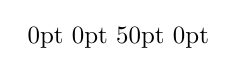
\begin{tikzpicture}[semithick]
\node[anchor=south west,inner sep=0pt,outer sep=0pt] at (0,0) {\scalebox{0.9}{\clipbox{0pt 0pt 50pt 0pt}{\usebox\deadlockExampleOne}}};
\end{tikzpicture}
\end{center}

\vskip1em

No transaction involved in a deadlock can continue.
\end{frame}

%
% -----------------------------------------------
%
\begin{frame}

\vskip1em

Detecting deadlocks with the \textbf{\alert{``waits-for'' graph}} of a set of running transactions:
\begin{itemize}[-,noitemsep,topsep=-5pt]
\item Nodes are transactions.
\item Add an edge $T_i \rightarrow T_j$ if $T_i$ is locked waiting for an element that $T_j$ holds.
\end{itemize}

\textbf{Theorem:} a set of transactions is in deadlock if (and only if) their waits-for graph contains a cycle.

\vskip1.5em

\begin{columns}[onlytextwidth]
\begin{column}{0.5\textwidth}
\resizebox{\textwidth}{!}{\clipbox{0pt 0pt 50pt 0pt}{\usebox\deadlockExampleOne}}
\end{column}
\begin{column}{0.3\textwidth}
\scalebox{0.75}{%
\begin{tikzpicture}[->,>=stealth',shorten >=1pt,auto,node distance=2.8cm,semithick]  
  \node[state] 	(1)                {$T_1$};
  \node[state]  (2) [right of=1]   {$T_4$};
  
  \path[->] 
  (1) edge [bend left] (2)
  (2) edge [bend left] (1);
\end{tikzpicture}}
\end{column}
\end{columns}
\end{frame}


\newsavebox\waitsForGraph
\savebox{\waitsForGraph}{%
\begin{tikzpicture}[->,>=stealth',shorten >=1pt,auto,node distance=2cm,semithick]
  \node[state] 	(3)                {$T_3$};
  \node[state]  (2) [right of=3]   {$T_2$};
  \node[state]  (1) [right of=2]   {$T_1$};
  \node[state]  (4) [above of=1]   {$T_4$};
  
  \path[->] 
  (3) edge (2)
  (2) edge (1)
  (1) edge [bend left] (3)
  (4) edge (1);
\end{tikzpicture}}

%
% -----------------------------------------------
%
\begin{frame}
\begin{center}
\scalebox{0.75}{\usebox\waitsForGraph}
\end{center}

\vskip2em

Note that a transaction can be in deadlock even if it is \textbf{not} part of the cycle.

In the example above, $T_4$ is also deadlocked because it cannot proceed until $T_1$ releases the locks on the elements it needs.

\end{frame}


%
% -----------------------------------------------
%
\begin{frame}{Breaking a deadlock}
\begin{columns}[onlytextwidth]
\begin{column}{0.65\textwidth}
Once a deadlock is detected the DBMS must pick one transaction in the cycle to \textbf{rollback}, allowing the others to continue (hopefully to completion).
\end{column}
\begin{column}{0.35\textwidth}
\resizebox{\textwidth}{!}{\usebox\waitsForGraph}
\end{column}
\end{columns}

But which one?
\begin{itemize}[-,noitemsep,topsep=-5pt]
\item The one holding up the most other transactions?
\item The one \textbf{closest to completion}?
\item The one \textbf{most recently started}?
\item The one from the user with \textbf{lowest priority}?
\end{itemize}

\vskip1em

It is up to the \textbf{database administrator} to implement whichever policy the organization decides to adopt.
\end{frame}

%
% -----------------------------------------------
%
\begin{frame}{Practical issues with locking}

Deadlocks can be avoided if the DBMS can impose a strict ordering on the database elements. But this is hard to do in practice, especially with transactions that insert new elements.

\alert{Maintaining the ``waits-for'' graph can be costly} (e.g., when there are thousands of concurrent transactions running). 
\begin{itemize}[-,topsep=-0.5em]
\item
Some systems \blue{monitor the CPU usage} of the transactions; if a transactions stops using the CPU, assume it is deadlocked.
\end{itemize}

\vskip1em

An \alert{exclusive lock} on a database element implies locks on \alert{\emph{all indexes}} defined over that element. 
\begin{itemize}[-,topsep=-0.5em]
\item Locking just some nodes of the B+-tree is possible, but tricky to implement.
\end{itemize}


\end{frame}


%%%%% ----------------- timestamps

%
% -----------------------------------------------
%

\section{Optimistic Concurrency Control with timestamps}

\begin{frame}

\vskip2em

The approach with optimistic concurrency control is to \alert{\textbf{monitor} the transactions as they execute}, intervening only when a problem has occurred or might occur.

The monitoring is based on when the transactions are accepted by the system. 
\begin{itemize}[-,topsep=-0.5em]
\item Each transaction gets a unique and immutable timestamp \blue{\TS{i}} based on the time it started.
\end{itemize}

\vskip1em
\begin{block}{Serializable schedules and timestamps}
Let $T_1,\ldots, T_n$ be a schedule where \TS{1} $< \cdots <$ \TS{n}. 

\vskip1em
Note that the schedule will be \emph{seriazable} if
whenever transactions $T_i$ and $T_j$ perform conflicting operations on the same element (i.e., at least one of them writes the element), if $i<j$ then $T_i$ performs its operation \textbf{before} $T_j$. 
\end{block}
\end{frame}


\begin{frame}

\textbf{Data structures needed for monitoring}


Recall that each transaction $T_i$ gets a \emph{unique} and immutable timestamp \blue{\TS{i}}, e.g., corresponding to its start time.

In order to know what transactions have been doing, the transaction monitor records the following information, for every element in use by an active transactions:
\begin{itemize}[-,noitemsep,topsep=-5pt]
\item \blue{\RT{X}}: timestamp of the transaction that most recently read \texttt{X};
\item \blue{\WT{X}}: timestamp of the transaction that most recently wrote \texttt{X};
\item \blue{\CT{X}}: bit indicating if the most recently written value of \texttt{X} has been committed to disk.
\end{itemize}

\vskip2em

These data structures allow the transaction monitor to detect non-serializable schedules!

\end{frame}

%
% -----------------------------------------------
%
\begin{frame}

Transactions send the following requests to the transaction monitorblue:\\
\begin{itemize}[-,noitemsep,topsep=-5pt]
 \item \R{i}{X} / \W{i}{X}:
 \item \C{i} / \A{i}
\end{itemize}

\vskip1em

The transaction monitor responds with one of the following:
\begin{itemize}[-,noitemsep,topsep=-5pt]
\item \blue{\textbf{grant}} the request: the operation proceeds;
\item \blue{\textbf{deny}} the request: the transaction is \underline{rolled back} (restarted, from scratch, with a new timestamp);
\item \blue{\textbf{delay}} the request: the transaction is put on hold until the scheduler can decide if it is safe to grant the request.
\end{itemize}

\vskip1em

Note that a request is denied only when the transaction monitor knows that granting the request would cause problems (e.g., break serializability).

\end{frame}

%
% -----------------------------------------------
%
\begin{frame}{Timestamp-based scheduling}

\begin{columns}
\begin{column}{0.5\textwidth}

\scalebox{0.75}{\begin{minipage}{1.3\textwidth}%
\begin{algorithm}[H]
\begin{algorithmic}[1]
\caption{Handling \R{i}{X} request by transaction $T_i$}
	\If {\TS{i} $<$ \WT{X}} \Comment{read too late!}
		\State \blue{deny} request; \underline{rollback} $T_i$
	\Else
		\If{\CT{X} is true \textbf{or} \TS{i}=\WT{x}}
			\State \blue{grant} request;
			\If{\TS{i} $>$ \RT{X}}
				\State \RT{X} = \TS{i}
			\EndIf
		\Else
			\State \blue{delay} request; put $T_i$ \underline{on hold}
		\EndIf
	\EndIf
\end{algorithmic}
\end{algorithm}
\end{minipage}}

\end{column}
\begin{column}{0.5\textwidth}

\scalebox{0.75}{\begin{minipage}{1.3\textwidth}%
\begin{algorithm}[H]
\begin{algorithmic}[1]
% \label{alg:write}
\caption{Handling \W{i}{X} request by transaction $T_i$}
	\If {\TS{i} $<$ \RT{X}} \Comment{write too late!}
		\State \blue{deny} request; \underline{rollback} $T_i$
	\Else
		\If{\TS{i} $\geq$ \WT{X}}
			\State \blue{grant} request; \underline{write} \texttt{X}
			\State set \WT{X} = \TS{i} and \CT{X} = false
		\Else
			\If {\CT{X} is true}
				\State do nothing; let $T_i$ continue
			\Else
				\State\label{delay_write} \blue{delay} request; put $T_i$ \underline{on hold}
			\EndIf
		\EndIf
	\EndIf
\end{algorithmic}
\end{algorithm}
\end{minipage}}

\end{column}
\end{columns}

\end{frame}

%
% -----------------------------------------------
%
\begin{frame}

\scalebox{0.75}{\begin{minipage}{\textwidth}%
\begin{algorithm}[H]
\begin{algorithmic}[1]
\caption{Handling \C{i} request by transaction $T_i$}
	\ForEach {element \texttt{X} written by $T_i$}
		\State set \CT{X} = true
		\ForEach {transaction $T_j$ waiting to read/write \texttt{X}}
			\State \blue{grant} $T_j$'s request; let $T_j$ continue
		\EndFor
	\EndFor
\end{algorithmic}
\end{algorithm}
\end{minipage}}

\scalebox{0.75}{\begin{minipage}{\textwidth}%
\begin{algorithm}[H]
\begin{algorithmic}[1]
\caption{Handling \A{i} request by transaction $T_i$}
	\ForEach {element \texttt{X} written by $T_i$}
		\ForEach {transaction $T_j$ waiting to read/write \texttt{X}}
			\State \underline{re-evaluate} $T_j$'s request with the current timestamps
		\EndFor
	\EndFor	
\end{algorithmic}
\end{algorithm}
\end{minipage}}
\end{frame}

%
% -----------------------------------------------
%

\newsavebox\TimeStampslostUpdateTimeline
\savebox{\TimeStampslostUpdateTimeline}{%
\footnotesize
\begin{tabular}{ll|rr||l}
$T_1$ --- \alert{\TS{1} = 100} & $T_2$ --- \alert{\TS{2} = 150} & \texttt{A} & \texttt{B} \\
\hline
& & 75 & 40   \\
\READ{A}{v}; \ASSIGN{v}{v-20} & & & &\RT{A}=100   \\
\WRITE{A}{v} & & 55 & & \WT{A} = 100; \CT{A}=false\\
\READ{B}{v}; \ASSIGN{v}{v+20} & & & &  \RT{B}=100\\
& \READ{B}{t}; \ASSIGN{t}{t*1.1} & & &  \alert{\RT{B}=150} \\
& \WRITE{B}{t} & & 44 & \WT{B}=150; \CT{B}=false\\
& \COMMIT & & \alert{44} & \CT{B}=true\\
\WRITE{B}{V} & & & & \DENY \\
\ROLLBACK & & \alert{75}&\\
\end{tabular}
}

\begin{frame}

Here's how timestamping avoids the ``lost update'' problem:

\begin{center}
\scalebox{0.9}{\usebox{\TimeStampslostUpdateTimeline}}
\end{center}

\vskip1em

Because \TS{1} $<$ \TS{2}, once $T_2$ writes \lstinline!B!, $T_1$ can no longer overwrite it.

Also, note that the new value of \lstinline!A! written by $T_1$ is not yet committed, so that change is not made permanent.

\end{frame}

\begin{frame}

Recall that with Strict 2PL, during a race condition, the transaction that acquires the lock first is allowed to continue (slide~\ref{lostUpdateWithTwoPL}).

\vskip2em

\begin{center}
\scalebox{0.75}{\usebox{\TimeStampslostUpdateTimeline}}
\end{center}

\vskip1em

With timestamping, on the other hand, every request is evaluated individually: Even though $T_1$ was granted the read on \lstinline!B! before $T_2$ started, that does not mean $T_1$ has priority.

For this reason, the request by $T_1$ is often called a ``write too late'' or ``write out of order''.

\end{frame}


\newsavebox\TimeStampslostUpdateTimelineHold
\savebox{\TimeStampslostUpdateTimelineHold}{%
\footnotesize
\begin{tabular}{ll|rr||l}
$T_1$ --- \alert{\TS{1} = 100} & $T_2$ --- \alert{\TS{2} = 150} & \texttt{A} & \texttt{B} \\
\hline
& & 75 & 40   \\
\READ{A}{v}; \ASSIGN{v}{v-20} & & & &\RT{A}=100   \\
\WRITE{A}{v} & & 55 & & \WT{A} = 100; \CT{A}=false\\
\READ{B}{v}; \ASSIGN{v}{v+20} & & & &  \RT{B}=100\\
& \READ{B}{t}; \ASSIGN{t}{t*1.1} & & &  \alert{\RT{B}=150} \\
& \WRITE{B}{t} & & 44 & \WT{B}=150; \CT{B}=false\\
\WRITE{B}{V} & & & & \DELAY \\
$\vdots$ & & & &
\end{tabular}
}

\begin{frame}

But what if $T_2$ had not yet committed?

\vskip1em

\begin{center}
\scalebox{0.9}{\usebox{\TimeStampslostUpdateTimelineHold}}
\end{center}

In this case, the transaction monitor does not know yet if the write requested by $T_1$ is valid or not: If $T_2$ later on aborts, $T_1$ should be allowed to write its value. If $T_2$ commits, $T_1$ is rolled back.

\end{frame}


\newsavebox\TimestampingInconsistentAnalysisTimeline
\savebox{\TimestampingInconsistentAnalysisTimeline}{%
\footnotesize
\begin{tabular}{ll|rr||l|l}
$T_1$ --- \alert{\TS{1} = 100} & $T_3$ --- \alert{\TS{3} = 200} & \texttt{A} & \texttt{B} & \lstinline[style=SQL]!SUM! &  \\
\hline
 & & 75 & 40 & \\
\READ{A}{v};  & & & & & \RT{A}=100\\
\ASSIGN{v}{v-20} & & & & \\
& \READ{A}{t};& & & & \RT{A}=200\\
& \ASSIGN{sum}{t} & & & 75 \\
\WRITE{A}{v} & & & & & \DENY\\
\ROLLBACK & & & &\\
& \READ{B}{t}; & & & & \RT{B}=200\\
& \ASSIGN{sum}{sum+t} & & & \alert{115}\\
\end{tabular}
}

\begin{frame}
Here's how timestamping avoids the ``inconsistent analysis'' problem:

\begin{center}
\scalebox{0.9}{\usebox{\TimestampingInconsistentAnalysisTimeline}}
\end{center}

\vskip1em

Again, even though $T_1$ started before $T_2$ (note their timestamps), that does not mean it has priority. 

Transactions are allowed to run until they make an invalid request.

\end{frame}

%
% -----------------------------------------------
%

\newsavebox\TimestampsDirtyReadTimeline
\savebox{\TimestampsDirtyReadTimeline}{%
\footnotesize
\begin{tabular}{ll|rr||l}
$T_1$ --- \alert{\TS{1} = 100} & $T_2$ --- \alert{\TS{2} = 150} & \texttt{A} & \texttt{B} & \\
\hline
& & 75 & 40 & \\
\READ{A}{v}; \ASSIGN{v}{v-20} & & & & \RT{A}=100\\
\WRITE{A}{v} & & 55 & & \WT{A}=100; \CT{A}=false\\
& \READ{B}{t}; \ASSIGN{t}{t*1.1} & & & \RT{B}=150\\
& \WRITE{B}{t} & &  44 & \WT{B}=150; \CT{B}=false\\
\READ{B}{v} & & & & \DELAY\\
& \ABORT & & \alert{40} & \\
\READ{B}{v}; \ASSIGN{v}{v+20} & & & & \RT{B}=100;\\
\WRITE{B}{v} & & & 60 & \WT{B}=100; \CT{B}=false\\
\COMMIT & & & \\
& & 55 & 60 & \CT{A}=true; \CT{B}=true \\
\end{tabular}
}

\begin{frame}

Here's how timestamping avoids the ``dirty read'' problem:

\begin{center}
\scalebox{0.9}{\usebox{\TimestampsDirtyReadTimeline}}
\end{center}

When $T_1$ attempts to read \lstinline!B! (again, too late), the transaction manager puts it on hold until the fate of $T_2$ is decided.

When $T_2$ aborts, $T_1$ is allowed to continue, reading the old value for that element.
\end{frame}

\section{Long-running transactions and snapshot isolation}


\newsavebox{\longRunningNRRexample}
\savebox{\longRunningNRRexample}{
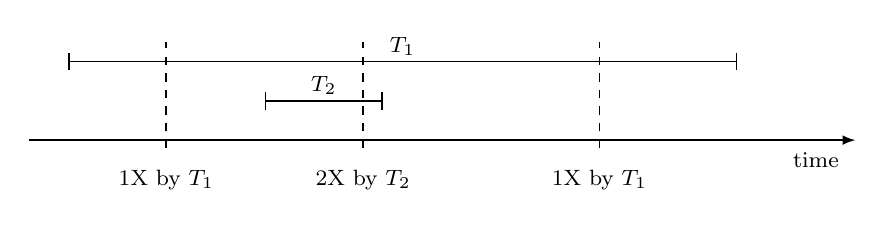
\begin{tikzpicture}[semithick,every node/.append style={font=\footnotesize}]
\begin{scope}[>=latex]
\draw [->] (0,1.5) -- (10.5,1.5); \node (caption) at (10,1.25) {time};
\draw [|-|] (0.5,2.5) -- (9,2.5) node [midway,yshift=-5pt,label=above:{$T_1$}] {};
\draw [|-|] (3,2) -- (4.5,2) node [midway,yshift=-5pt,label=above:{$T_2$}] {};
\end{scope}

\draw[dashed] (1.75,1.4) -- (1.75,2.75); % t1 reads (X)
\node [] at (1.75,1.0) {\R{1}{X} by $T_1$};

\draw[dashed] (4.25,1.4) -- (4.25,2.75); % t2 writes (X)
\node [] at (4.25,1.0) {\W{2}{X} by $T_2$};

\draw[dashed] (7.25,1.4) -- (7.25,2.75); % t1 read (X)
\node [] at (7.25,1.0) {\R{1}{X} by $T_1$};
\end{tikzpicture}}


\begin{frame}

Consider transactions $T_1$ and $T_2$ that both need to write to a database element \lstinline[style=SQL]!X!, and the following timeline corresponding to running them \textbf{without} any concurrency control:

\vskip2em

\begin{center}
\usebox{\longRunningNRRexample}
\end{center}

\vskip2em

If we use locking, $T_2$ must wait a long time (as $T_1$ started first).

If we use time-stamping, $T_1$ will be rolled back, after computing for a long time.

\end{frame}

%
% -----------------------------------------------
%
\begin{frame}{Multi-Version Concurrency Control (MVCC)}

Instead of overwriting the element, a write operation creates a \textbf{new version}, used by transactions with that timestamp (or higher).

\vskip1em

\begin{center}
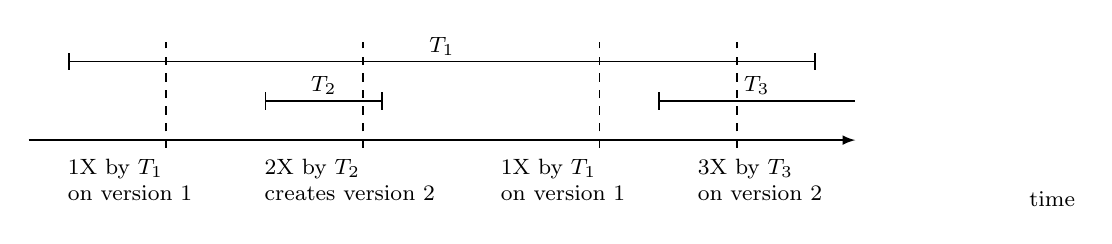
\begin{tikzpicture}[semithick,every node/.append style={font=\footnotesize}]
\begin{scope}[>=latex]
\draw [->] (0,1.5) -- (10.5,1.5); \node (caption) at (13,0.75) {time};
\draw [|-|] (0.5,2.5) -- (10,2.5) node [midway,yshift=-5pt,label=above:{$T_1$}] {};
\draw [|-|] (3,2) -- (4.5,2) node [midway,yshift=-5pt,label=above:{$T_2$}] {};
\end{scope}

\draw[dashed] (1.75,1.4) -- (1.75,2.75); % t1 reads (X)
\node [text width=2.5cm] at (1.75,1.0) {\R{1}{X} by $T_1$\\on version 1};

\draw[dashed] (4.25,1.4) -- (4.25,2.75); % t2 writes (X)
\node [text width=2.5cm] at (4.25,1.0) {\W{2}{X} by $T_2$\\\alert{creates version 2}};

\draw[dashed] (7.25,1.4) -- (7.25,2.75); % t1 read (X)
\node [text width=2.5cm] at (7.25,1.0) {\R{1}{X} by $T_1$\\on version 1};

\only<2- | handout:1>{
\draw [|-] (8,2) -- (10.5,2) node [midway,yshift=-5pt,label=above:{$T_3$}] {};
\draw[dashed] (9,1.4) -- (9,2.75); % t1 read (X)
\node [text width=2.5cm] at (9.75,1.0) {\R{3}{X} by $T_3$\\on \alert{version 2}};
}
\end{tikzpicture}
\end{center}

\vskip1em

In this method, each transaction runs on a ``snapshot'' of the database, consistent with the time the transaction started\footnote{\url{https://en.wikipedia.org/wiki/Snapshot_isolation}}.
\end{frame}


\begin{frame}

But snapshot isolation re-introduces the ``lost update'' problem:

\vskip1em

\begin{center}
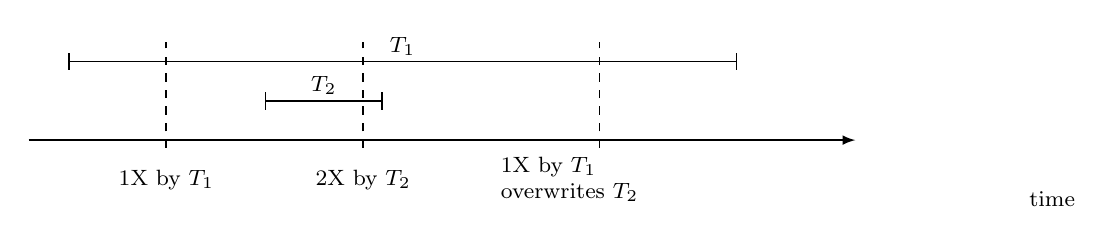
\begin{tikzpicture}[semithick,every node/.append style={font=\footnotesize}]
\begin{scope}[>=latex]
\draw [->] (0,1.5) -- (10.5,1.5); \node (caption) at (13,0.75) {time};
\draw [|-|] (0.5,2.5) -- (9,2.5) node [midway,yshift=-5pt,label=above:{$T_1$}] {};
\draw [|-|] (3,2) -- (4.5,2) node [midway,yshift=-5pt,label=above:{$T_2$}] {};
\end{scope}

\draw[dashed] (1.75,1.4) -- (1.75,2.75); % t1 reads (X)
\node [] at (1.75,1.0) {\R{1}{X} by $T_1$};

\draw[dashed] (4.25,1.4) -- (4.25,2.75); % t2 writes (X)
\node [] at (4.25,1.0) {\W{2}{X} by $T_2$};

\draw[dashed] (7.25,1.4) -- (7.25,2.75); % t1 read (X)
\node [text width=2.5cm] at (7.25,1.0) {\W{1}{X} by $T_1$\\\alert{overwrites} $T_2$};
\end{tikzpicture}
\end{center}

\vskip1em

If $T_1$ \alert{\textbf{writes}} element \lstinline[style=SQL]!X! that will overwrite the update by $T_2$.

This can lead to inconsistencies, as other values written by $T_2$ could have been calculated based on the value of \lstinline[style=SQL]!X! in its snapshot.

Different DBMSs handle this problem differently. Often, the solution is to let the DBA or the application decide how to handle the problem.

\end{frame}


%
% -----------------------------------------------
%
